\documentclass[article]{report} % Type of document

\usepackage[utf8]{inputenc}    		 	% Encoding
\usepackage[english]{babel}			% Language
\usepackage{geometry}           			% Page margin
\usepackage{graphicx}           			% For images
\usepackage{newcent}            			% Font
\usepackage{color}              			% Colors
\usepackage{listings}           			% Lists
\usepackage[footnote, nolist]{acronym}	% Acronyms
\usepackage[absolute, overlay]{textpos}	% Text positioning

\usepackage{fancyhdr}          			 % We might have a need for them
\usepackage{float}
\usepackage{tabularx}

\usepackage{latexsym}
\usepackage{pdfpages}
\usepackage{tikz}
\usepackage{ifthen}
\usepackage{wrapfig}
\usepackage{textcomp}
\usepackage{multicol}

\setlength{\columnsep}{1cm}
\setlength{\TPHorizModule}{\paperwidth}	% Used for textblock
\setlength{\TPVertModule}{\paperheight}	% Used for textblock

\title {Oral Presentation 1}
\parskip = 0.25cm              % Summary options (spaces between lines)

% Margin
\geometry{tmargin=2.5cm, bmargin=1.5cm, lmargin=2.5cm, rmargin=2cm}

\definecolor{blue}{rgb}{0.13,0.29,0.46}
\definecolor{red}{rgb}{1,0,0}
\definecolor{couleur_titre}{rgb}{0.20, 0.45, 0.80}
\definecolor{couleur_nom}{rgb}{0.11, 0.6, 0.18}

\renewcommand{\labelitemi}{$\bullet$}
\renewcommand{\contentsname}{Table of contents}

% Title at the top of the page
\pagestyle{fancyplain} \chead{}\lhead{\textit{Team Dedalus}} \rhead{\textcolor{couleur_titre}{\emph{\textit{Project: SkyLands}}}}

\title {Book of specifications}
\author {Romain\and Renaud\and Aenora\and Erwan}
\date {}

%
% Document
%
\begin{acronym}
	\acro{OO}{Oriented-Object}
	\acro{RTS}{Real Time Strategy}
	\acro{FPS}{First Person Shooter}
	\acro{Mogre}{Managed Object-Oriented Graphics Rendering Engine}
	\acro{API}{Application Progamming Interface}
	\acro{GUI}{Graphical User Interface}
	\acro{MyGUI}{Multilayer and overlappable GUI System}
	\acro{IDE}{Integrated Developement Environment}
	\acro{AI}{Artificial Intelligence}
	\acro{NPC}{Non Player Character}
	\acro{UML}{Unified Modeling Language}
	\acro{PHP}{PHP : Hypertext Preprocessor}
	\acro{ORM}{Object-Relational Mapping}
	\acro{MVC}{Model View Controller}
	\acro{OGRE}{Object-Oriented Graphics Rendering Engine}
\end{acronym}
\begin{document}
		\thispagestyle{empty}
  			\begin{titlepage} 
						\vspace*{1cm} 
  					\begin{center} 
  							{\huge{\textsc{1st Oral} \\ ~ \\{\large From}\\ ~\\ Team \\  ~ \\ }}
	  						\includegraphics[width = 14cm]{Images/Dedalus.png}
							\\ ~ \\ ~ \\ ~ \\ ~ \\ ~ \\ ~ \\ ~ \\ ~ \\ ~ \\ ~ \\ ~ \\ ~ \\ ~ \\ ~ 
						\end{center}
  					\hfill {\large Romain \textsc{Biessy}}
  					\hfill {\large Renaud \textsc{Gaubert}}
  					\hfill {\large Aenora \textsc{Tye}}
  					\hfill {\large Erwan  \textsc{Vasseure}}
  			\end{titlepage} 

  	\tableofcontents
  		\pagenumbering{arabic}
  		\newpage
		
		\chapter{\textcolor{blue}{Introduction}}
 			An ambitious 3d game such as ours requires a lot of work, to give you an example we spent not less than 100 hours each on the project since october also our project actually counts 120 000 characters and 15 000 lines of codes with not less than a 100 files.

 			Of course this would be meaningless if we wrote bad code however while not having the pretention to say that we write good code we have the pretention to say that 
 			we do note write bad code.

 			Throughout this report we will try hilight the fact that our work has payed and we already have good base to proceed without worries the developpement of our game.

 			%Logo Skylands Ici


								
  		\chapter{\textcolor{blue}{Gameplay}}
			\section{RTS, FPS \& minecraft-like}

			\section{Scenario}
				As time went on, we thought of a better scenario than the one elaborated for the book of specifications. 
				And we came up with two scenarios of our own : 

				\begin{description}
					\item In the second part of the 24th century, human race is at war, you are a soldier, sent to unknown planet which seems to be only composed
						with flying islands and your goal is to take the island right under the ennemy's nose !
					\item Un 2nd scénario ici
				\end{description} 

		\chapter{\textcolor{blue}{Character}}
			\section{Mesh}
\paragraph
				At the beginning we were using the mogre mascot called Sinbad. It was useful since it has predefined animations; the drawback is that he doesn't have the right size, and it isn't made for being integrated in a cubic world. After that Aenora and Erwan made a few different characters in blender, a 3d software. We encountered difficulties while trying to implement the new mesh file and its animations into the mogre engine. Some of the character textures were made with the UV mapping technique.
			\section{Move}
				We can move our character with the directional arrows or the WASD keys. Animations start by pressing one of these keys. There are four animations; two for the walking loop and two for the idle loop. Erwan integrated the keys manager, inspiring himself from the MOIS manager provided by mogre.\\

An issue Erwan encountered is the rotation of the player because we have a 3D world. If we needed some advanced rotations we would had to use quaternions, a powerful but non-intuitive mathematical tool similar to matrice in 4 dimensions. Fortunately an easier way is to decompose the rotation within the 3 axes (x, y, z). This is way simpler since we only need to rotations : yawing the player (around the y-axis) switch the horizontal movement of the mouse and pitching the camera (around the x-axis) switch the vertical movement of the mouse. Erwan implemented the rotation as well.
			\section{Animation}
				Romain intergrated a fade for the transitions of animation. Basicaly, animations have a weight between 0 and 1, 0 is no animation and 1 is the full animation, 0.5 would be that animation, but with a lower amplitude. The fade is made by downcreasing the old animation's weight to 0, while increasing the new one to 1. This method garantees a smooth transition between all the animations even if they are stopped before their end in game.

			\section{Collision}
				The hit-box of the character is represented by the 8 points of a parallelepiped rectangle. To test collision we look at the type of block around the character. For instance if we want to test the feet collisions, we get the type of the block under the character, using the 4 lowest points. For the next presentation, Romain will have to finish all the collisions test.

			\section{Camera}
				We can switch among two cameras in our game the first person one and the debug one. The first person camera is following the player, it just has to be pitch depending on the mouse. The debug camera isn't supposed to be seen by a player, thought it is very useful for us since it's a free camera detached from the player. Thus, we can see the whole world and the player with its animations. They have been both implemented by Romain.

			\section{What must be done}
		\chapter{\textcolor{blue}{Graphic engine and terrain}}
			\section{Ogre3D}
				A 3D world is at first sight more complex than you could imagine.The player moves via an FPS (Fisrt Person Shooter) type camera. While its position in space is given by a Vector3 (3 floats). The orientation of the camera uses rotations about the X and Y axes: this is called respectively the yaw and pitch (the roll, rotation around the Z axis is not useful in our cases).
			\begin{figure}[h]
				
\includegraphics[width=11cm,   height=7cm]{Images/axis.png}
				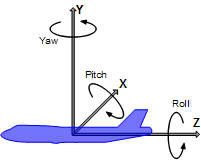
\includegraphics[width=6.5cm]{Images/Rotations.jpeg}
			\end{figure}
			
			A trick to find if the rotation you want to apply is a positive rotation or a negative rotation is the following : \\
			\begin{figure}[h]
				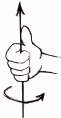
\includegraphics[]{Images/RotationsPositive.png}
			\end{figure}
			\begin{textblock}{0.628}(0.250, 0.825)
							\noindent  Using your right hand as a guide: point your thumb in the direction of an axis, curl your remaining fingers. The direction of the curl matches the positive rotation around that axis
						\end{textblock}
			\section{Terrain Generation}
				When creating the terrain architecture we had the goal to separate the terrain in multiple arrays which we called chunks. Thus, when we will be able to save the terrain, we won't save it in a single file. Also this permits us to later, dynamically load the terrain chunks by chunks and not as a single entity. \\

				The terrain Hierarchy is as follows : World contains a few islands which themselves contains a dictionary of chunks which contains a 16 * 16 * 16 array of blocks. It follows this chart : 
				\begin{figure}[h]
					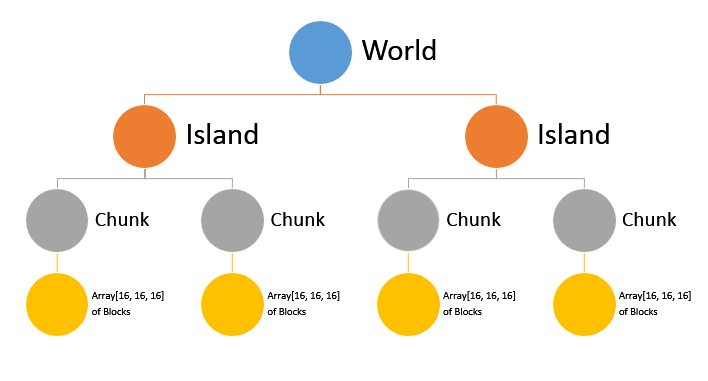
\includegraphics[width=18cm]{Images/WorldHierarchy.png}
					\begin{center}\it test \end{center}
				\end{figure}

				The terrain itself is generated when we create the island, using a perlin 3d algorith we go through all the blocks in the islands (3 simple for) and for each block, we compute it's perlin noise value and check if it is superior to 0 to display it.
				
			\section{Terrain Display}

			\section{Solved Issues and Unsolved}			

			\section{What must be done}
	\chapter{\textcolor{blue}{Conclusion}}

					 

					


				\begin{center}
					
\includegraphics[width = 16cm]{Images/Islands_Title.png}
				\end{center}     	     		
\end{document}